\begin{frame}
\frametitle{(Classical!) Circuit Hamiltonian}
\begin{columns}
  \begin{column}{0.3\textwidth}
    \begin{figure}
      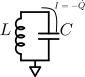
\includegraphics[scale=1.2]{LC_oscillator_annotated.pdf}
    \end{figure}
  \end{column}
  \begin{column}{0.7\textwidth}
    $Q \equiv $ charge on capacitor. $\Phi \equiv$ flux in inductor.
  \end{column}
\end{columns}

\begin{columns}[t]
  \begin{column}{0.4\textwidth}
    \textbf{Kirchoff's laws}
    \begin{align*}
      -\dot{Q} =& \Phi/L \quad Q/C = V = \dot{\Phi} \\
      \ddot{\Phi} =& -\omega_0 \Phi \\
      \Phi(t) =& M \cos(\omega_0 t + \phi) \\
    \end{align*}
  \end{column}
  \begin{column}{0.4\textwidth}
    \textbf{Hamiltonian}
    \begin{align*}
      H =& \frac{Q^2}{2C} + \frac{\Phi^2}{2L} \\
      \dot{Q} =& - \frac{\partial H}{\partial \Phi} = -\frac{\Phi}{L} \\
      \dot{\Phi} =& \frac{\partial H}{\partial Q} = \frac{Q}{C} \\
      \ddot{\Phi} =& - \omega_0^2 \Phi \, .
    \end{align*}
  \end{column}
\end{columns}
\only<2->{Quantum case?} \only<3->{$\mathcolor{red}{[\Phi, Q] = i \hbar}$}
\end{frame}
